% questions.tex —— 2004 年·春季上海卷 · 题目内容片段（无答案）
% 由 tools/generate_projects.py 依来源总账自 2004/2004_数学真题_春季上海_试题.md 生成，勿手改（改源 MD 后重跑）


\gkpart{数学试卷}

\begin{gktip}
\textbf{来源说明}：按固定来源 PDF 及其可提取文字层转录，并目视核对两页原件。原件没有答案页；题目原文中的疑点按原样保留，不推测修订。固定 PDF 是 XeTeX 重排件，出版者、版次及上游来源链尚未核实；paper_id 仅用于本库内部固定字节绑定，不代表官方身份认证。

\textbf{图表说明}：第 6 题正三棱锥图、第 8 题五幅点阵变化图、第 11 题杨辉三角及第 20 题斜三棱柱图均见原件，已提供 TikZ 矢量源并通过独立图像复核及局部编译、渲染，不以栅格图入库。详见图表清单。本稿暂不作为正式 LaTeX 构建输入。
\end{gktip}

\gkpart{一、填空题}

\begin{question}
\gkti{1}若复数 $z$ 满足 $z(1+i)=2$，则 $z$ 的实部是 $\underline{\qquad}$。

\end{question}
\begin{question}
\gkti{2}方程 $\lg x+\lg(x+3)=1$ 的解 $x=\underline{\qquad}$。

\end{question}
\begin{question}
\gkti{3}在 $\triangle ABC$ 中，$a,b,c$ 分别是 $\angle A$、$\angle B$、$\angle C$ 所对的边。若 $\angle A=105^\circ$，$\angle B=45^\circ$，$b=2\sqrt{2}$，则 $c=\underline{\qquad}$。

\end{question}
\begin{question}
\gkti{4}过抛物线 $y^2=4x$ 的焦点 $F$ 作垂直于 $x$ 轴的直线，交抛物线于 $A$、$B$ 两点，则以 $F$ 为圆心、$AB$ 为直径的圆方程是 $\underline{\qquad}$。

\end{question}
\begin{question}
\gkti{5}已知函数 $f(x)=\log_3\left(\dfrac{4}{x}+2\right)$，则方程 $f^{-1}(x)=4$ 的解 $x=\underline{\qquad}$。

\Needspace{0.4\textheight}
\end{question}
\begin{question}
\gkti{6}如图，在底面边长为 $2$ 的正三棱锥 $V-ABC$ 中，$E$ 是 $BC$ 的中点。若 $\triangle VAE$ 的面积是 $\dfrac{1}{4}$，则侧棱 $VA$ 与底面所成角的大小为 $\underline{\qquad}$。（结果用反三角函数值表示。）
\nopagebreak[4]
\begin{center}% Q6：线型按原页复现。空间位置仅作示意，不按比例。
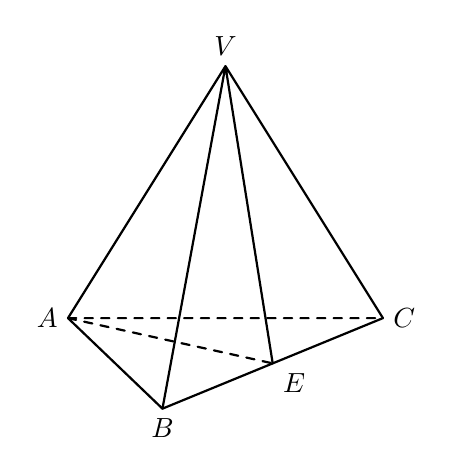
\begin{tikzpicture}[line cap=round,line join=round,thick]
  \coordinate (V) at (0,3.2);
  \coordinate (A) at (-2.0,0);
  \coordinate (B) at (-0.8,-1.15);
  \coordinate (C) at (2.0,0);
  \coordinate (E) at (0.6,-0.575);

  % Visible pyramid edges and the median in face VBC.
  \draw (V)--(A) (V)--(B) (V)--(C) (V)--(E);
  \draw (A)--(B)--(C);

  % Hidden rear base edge and the indicated segment AE.
  \draw[dashed] (A)--(C) (A)--(E);

  \node[above] at (V) {$V$};
  \node[left] at (A) {$A$};
  \node[below] at (B) {$B$};
  \node[right] at (C) {$C$};
  \node[below right] at (E) {$E$};
\end{tikzpicture}
\end{center}
\nopagebreak[4]
\end{question}
\begin{question}
\gkti{7}在数列 $\{a_n\}$ 中，$a_1=3$，且对任意大于 $1$ 的正整数 $n$，点 $(\sqrt{a_n},\sqrt{a_{n-1}})$ 在直线 $x-y-\sqrt{3}=0$ 上，则 $\displaystyle\lim_{n\to\infty}\dfrac{a_n}{(n+1)^2}=\underline{\qquad}$。

\Needspace{0.4\textheight}
\end{question}
\begin{question}
\gkti{8}根据下列 $5$ 个图形及相应点的个数的变化规律，试猜测第 $n$ 个图形中有 $\underline{\qquad}$ 个点。
\nopagebreak[4]
\begin{center}% Q8：逐点复现原页的五个空心圆点阵，不据此添加题目未给的几何条件。
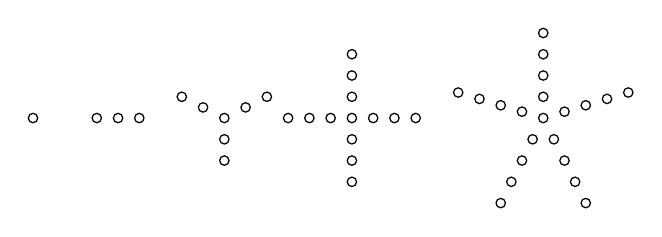
\begin{tikzpicture}[x=0.27cm,y=0.27cm,line width=0.45pt]
  \foreach \x/\y in {
    0/0,
    3/0,4/0,5/0,
    7/1,8/0.5,9/0,10/0.5,11/1,9/-1,9/-2,
    15/-3,15/-2,15/-1,15/0,15/1,15/2,15/3,
    12/0,13/0,14/0,16/0,17/0,18/0,
    24/4,24/3,24/2,24/1,
    20/1.2,21/0.9,22/0.6,23/0.3,24/0,25/0.3,26/0.6,27/0.9,28/1.2,
    23.5/-1,24.5/-1,23/-2,25/-2,22.5/-3,25.5/-3,22/-4,26/-4
  } {
    \draw[fill=white] (\x,\y) circle[radius=1.7pt];
  }
\end{tikzpicture}
\end{center}
\nopagebreak[4]
\end{question}
\begin{question}
\gkti{9}一次二期课改经验交流会打算交流试点学校的论文 $5$ 篇和非试点学校的论文 $3$ 篇。若任意排列交流次序，则最先和最后交流的论文都为试点学校的概率是 $\underline{\qquad}$。（结果用分数表示。）

\end{question}
\begin{question}
\gkti{10}若平移椭圆 $4(x+3)^2+9y^2=36$，使平移后的椭圆中心在第一象限，且它与 $x$ 轴、$y$ 轴分别只有一个交点，则平移后的椭圆方程是 $\underline{\qquad}$。

\Needspace{0.4\textheight}
\end{question}
\begin{question}
\gkti{11}如图，在由二项式系数所构成的杨辉三角形中，第 $\underline{\qquad}$ 行中从左至右第 $14$ 与第 $15$ 个数的比为 $2:3$。
\nopagebreak[4]
\begin{center}% Q11：忠实排出原页可见的杨辉三角前六行及行号。
\begin{tikzpicture}[x=0.78cm,y=0.62cm]
  \foreach \r in {0,...,5} {
    \node[anchor=east] at (-3.2,-\r) {第 \r 行};
  }
  \node at (0,0) {1};
  \node at (-0.5,-1) {1}; \node at (0.5,-1) {1};
  \node at (-1,-2) {1}; \node at (0,-2) {2}; \node at (1,-2) {1};
  \node at (-1.5,-3) {1}; \node at (-0.5,-3) {3};
  \node at (0.5,-3) {3}; \node at (1.5,-3) {1};
  \node at (-2,-4) {1}; \node at (-1,-4) {4}; \node at (0,-4) {6};
  \node at (1,-4) {4}; \node at (2,-4) {1};
  \node at (-2.5,-5) {1}; \node at (-1.5,-5) {5}; \node at (-0.5,-5) {10};
  \node at (0.5,-5) {10}; \node at (1.5,-5) {5}; \node at (2.5,-5) {1};
  \node[anchor=east] at (-2.5,-6) {$\cdots\cdots$};
  \node at (0,-6) {$\cdots\cdots$};
\end{tikzpicture}
\end{center}
\nopagebreak[4]
\end{question}
\begin{question}
\gkti{12}在等差数列 $\{a_n\}$ 中，当 $a_r=a_s$（$r\ne s$）时，$\{a_n\}$ 必定是常数数列。然而在等比数列 $\{a_n\}$ 中，对某些正整数 $r,s$（$r\ne s$），当 $a_r=a_s$ 时，非常数数列 $\{a_n\}$ 的一个例子是 $\underline{\qquad}$。

\end{question}
\gkpart{二、选择题}

\begin{question}
\gkti{13}下列函数中，周期为 $1$ 的奇函数是\mbox{（　　）}。

（A）$y=1-2\sin^2\pi x$　　（B）$y=\sin\left(2\pi x+\dfrac{\pi}{3}\right)$　　（C）$y=\tan\dfrac{\pi}{2}x$　　（D）$y=\sin\pi x\cos\pi x$

\end{question}
\begin{question}
\gkti{14}若非空集合 $M\subseteq N$，则“$a\in M$ 或 $a\in N$”是“$a\in M\cap N$”的\mbox{（　　）}。

（A）充分非必要条件　　（B）必要非充分条件　　（C）充要条件　　（D）既非充分又非必要条件

\end{question}
\begin{question}
\gkti{15}在 $\triangle ABC$ 中，有命题：① $\overrightarrow{AB}-\overrightarrow{AC}=\overrightarrow{BC}$；② $\overrightarrow{AB}+\overrightarrow{BC}+\overrightarrow{CA}=\vec{0}$；③ 若 $(\overrightarrow{AB}+\overrightarrow{AC})\cdot(\overrightarrow{AB}-\overrightarrow{AC})=0$，则 $\triangle ABC$ 为等腰三角形；④ 若 $\overrightarrow{AC}\cdot\overrightarrow{AB}>0$，则 $\triangle ABC$ 为锐角三角形。上述命题正确的是\mbox{（　　）}。

（A）①②　　（B）①④　　（C）②③　　（D）②③④

\end{question}
\begin{question}
\gkti{16}若 $p=a+\dfrac{1}{a}+2$（$a>0$），$q=\arccos t$（$-1\le t\le1$），则下列不等式恒成立的是\mbox{（　　）}。

（A）$p\ge\pi>q$　　（B）$p>q\ge0$　　（C）$4>p\ge q$　　（D）$p\ge q>0$

\end{question}
\gkpart{三、解答题}

\begin{question}
\gkti{17}在直角坐标系 $xOy$ 中，已知点 $P(2\cos x+1,\,2\cos 2x+2)$ 和点 $Q(\cos x,-1)$，其中 $x\in[0,\pi]$。若向量 $\overrightarrow{OP}$ 与 $\overrightarrow{OQ}$ 垂直，求 $x$ 的值。

\end{question}
\begin{question}
\gkti{18}已知实数 $p$ 满足不等式 $\dfrac{2x+1}{x+2}<0$，试判断方程 $z^2-2z+5-p^2=0$ 有无实根，并给出证明。

\begin{gktip}
\textbf{原文疑点}：原件印作“实数 $p$ 满足不等式”，但该不等式使用变量 $x$；本稿按原件保留，未将 $x$ 擅改为 $p$。该疑点影响题意解释，待取得可追溯的同版答案/勘误或其他直接来源后复核。
\end{gktip}

\end{question}
\begin{question}
\gkti{19}某市 $2003$ 年共有 $1$ 万辆燃油型公交车。有关部门计划于 $2004$ 年投入 $128$ 辆电力型公交车，随后电力型公交车每年的投入比上一年增加 $50\%$。试问：

（1） 该市在 $2010$ 年应该投入多少辆电力型公交车？

（2） 到哪一年底，电力型公交车的数量开始超过该市公交车总量的 $\dfrac{1}{3}$？

\Needspace{0.4\textheight}
\end{question}
\begin{question}
\gkti{20}如图，点 $P$ 为斜三棱柱 $ABC-A_1B_1C_1$ 的侧棱 $BB_1$ 上一点，$PM\perp BB_1$ 交 $AA_1$ 于点 $M$，$PN\perp BB_1$ 交 $CC_1$ 于点 $N$。

（1） 求证：$CC_1\perp MN$；

（2） 在任意 $\triangle DEF$ 中有余弦定理：$DE^2=DF^2+EF^2-2DF\cdot EF\cos\angle DFE$。拓展到空间，类比三角形的余弦定理，写出斜三棱柱的三个侧面面积与其中两个侧面所成的二面角之间的关系式，并予以证明。
\nopagebreak[4]
\begin{center}% Q20：按原图复现斜三棱柱的顶点、可见/隐藏棱及 P,M,N 辅助线。
% 投影为示意布局，不表达未给出的长度或角度。
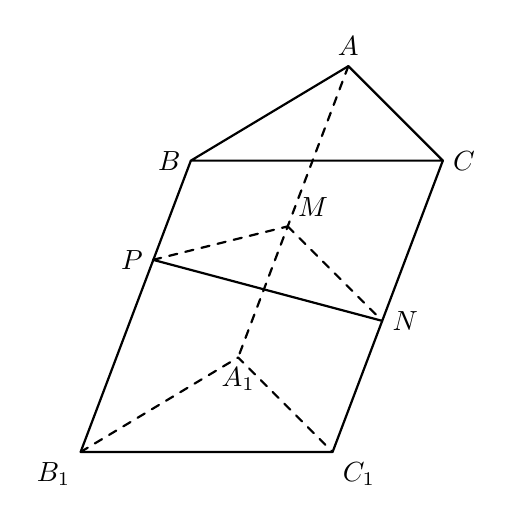
\begin{tikzpicture}[line cap=round,line join=round,thick]
  \coordinate (A)  at (2.0,4.0);
  \coordinate (B)  at (0.0,2.8);
  \coordinate (C)  at (3.2,2.8);
  \coordinate (A1) at (0.6,0.3);
  \coordinate (B1) at (-1.4,-0.9);
  \coordinate (C1) at (1.8,-0.9);
  \coordinate (P)  at (-0.48,1.54);
  \coordinate (M)  at (1.23,1.965);
  \coordinate (N)  at (2.43,0.765);

  % Upper face and visible prism edges.
  \draw (A)--(B)--(C)--(A);
  \draw (B)--(B1) (C)--(C1) (B1)--(C1);

  % Hidden back edge and rear triangular face.
  \draw[dashed] (A)--(A1) (B1)--(A1)--(C1);

  % Auxiliary construction shown in the original.
  \draw[dashed] (P)--(M) (M)--(N);
  \draw (P)--(N);

  \node[above] at (A) {$A$};
  \node[left] at (B) {$B$};
  \node[right] at (C) {$C$};
  \node[below] at (A1) {$A_1$};
  \node[below left] at (B1) {$B_1$};
  \node[below right] at (C1) {$C_1$};
  \node[left] at (P) {$P$};
  \node[above right] at (M) {$M$};
  \node[right] at (N) {$N$};
\end{tikzpicture}
\end{center}
\nopagebreak[4]
\end{question}
\begin{question}
\gkti{21}已知函数 $f(x)=|x-a|$，$g(x)=x^2+2ax+1$（$a$ 为正常数），且函数 $f(x)$ 与 $g(x)$ 的图象在 $y$ 轴上的截距相等。

（1） 求 $a$ 的值；

（2） 求函数 $f(x)+g(x)$ 的单调递增区间；

（3） 若 $n$ 为正整数，证明：$10^{f(n)}\cdot\left(\dfrac{4}{5}\right)^{g(n)}<4$。

\end{question}
\begin{question}
\gkti{22}已知倾斜角为 $45^\circ$ 的直线 $l$ 过点 $A(1,-2)$ 和点 $B$，$B$ 在第一象限，$|AB|=3\sqrt{2}$。

（1） 求点 $B$ 的坐标；

（2） 若直线 $l$ 与双曲线 $C:\dfrac{x^2}{a^2}-y^2=1$（$a>0$）相交于 $E$、$F$ 两点，且线段 $EF$ 的中点坐标为 $(4,1)$，求 $a$ 的值；

（3） 对于平面上任一点 $P$，当点 $Q$ 在线段 $AB$ 上运动时，称 $|PQ|$ 的最小值为点 $P$ 与线段 $AB$ 的距离。已知点 $P$ 在 $x$ 轴上运动，写出点 $P(t,0)$ 到线段 $AB$ 的距离 $h$ 关于 $t$ 的函数关系式。

\end{question}